\section{Flag 05 - Spoof (Curl)}

\paragraph{f2a29020ef3132e01dd61df97fd33ec8d7fcd1388cc9601e7db691d17d4d6188}
\begin{center}
    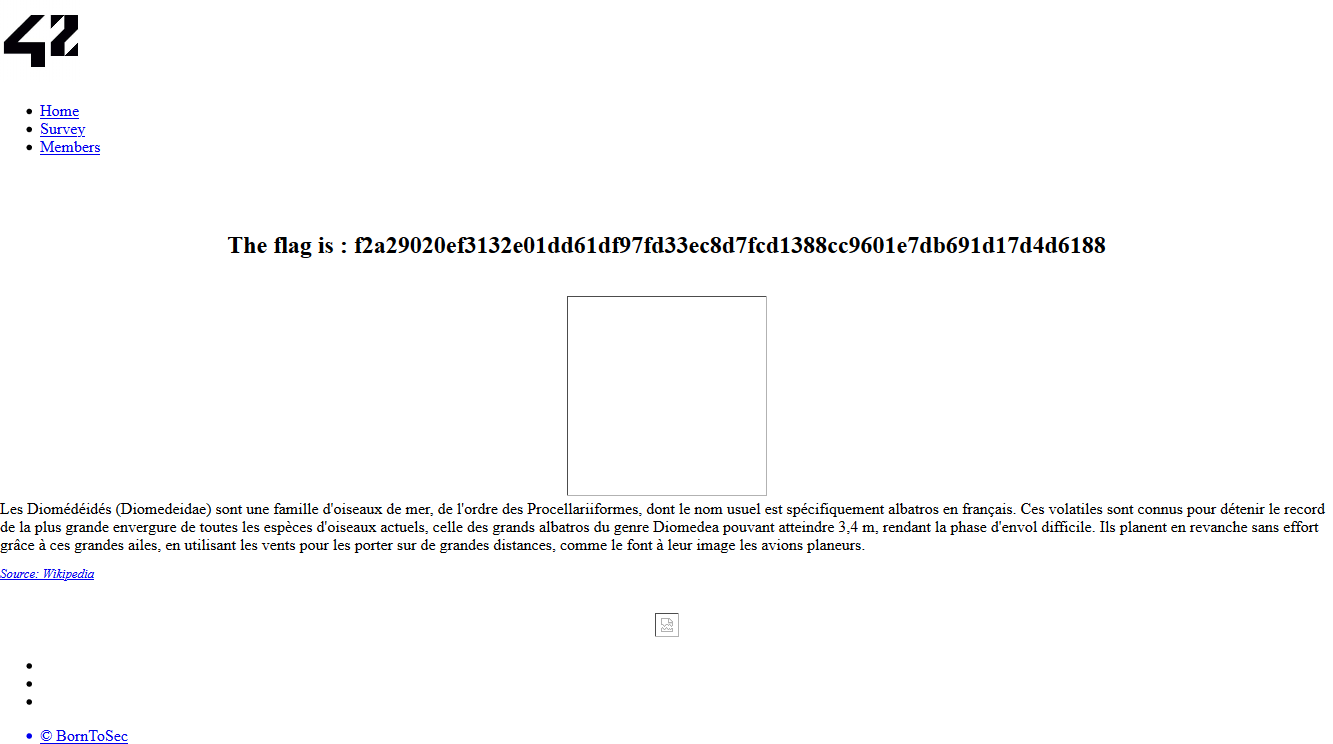
\includegraphics[width=0.5\textwidth]{08.Flag05/05-04.png}\\[0cm] 
\end{center}

\subsection{Vulnerability}

If you rely on the optional setting of HTTP Referrer of Agent, you will find yourself being tricked as this information can be faked. There is no real reason to require this information as Web Browsers are usually consistent in their display methods regardless.

\subsection{Location}

At the footer of 'http://<ip-address>:80/index.php' you will see text labelled `BornToSec`. Clicking on it will refer you to page

`http://<ip-address>:80/index.php?page=e43ad1fdc54babe674da7c7b8f0127bde61de3fbe01def7d00f151c2fcca6d1c`

\subsection{Method}

When you are on the page, you can object the Object Inspector. You will after going through the code, see that there are many comments embedded within. One that catches the eye is written as

```

<!- -

You must cumming from : "https://www.nsa.gov/" to go to the next step

- ->

```

If you keep scrolling you will see another comment that states:

```

<!- -

Let's use this browser : "ft\_bornToSec". It will help you a lot.

- ->

```

This is a big clue for anyone who successfully completed the PHP Bootcamp, specifically the day related to cURL. When using cURL, a person can refer themselves using agents.

This means we need to run a cURL script in our terminal. Here is our script:

```

ip="http://192.168.0.145"

curl -v -o sinkosi.html \

-e 'https://www.nsa.gov/' \

-A 'ft\_bornToSec' \

"\${ip}/index.php?page=e43ad1fdc54babe674da7c7b8f0127bde61de3fbe01def7d00f151c2fcca6d1c"\

```
\begin{itemize}
    \item ip = `<ip-address>` of your VM
    \item -v = [verbose](https://curl.haxx.se/docs/manpage.html\#-v) makes curl give output, useful for Debugging
    \item -e = [referer](https://curl.haxx.se/docs/manpage.html\#-e) sends the "Referer Page" information to the HTTP Server
    \item -A = [user-agent](https://curl.haxx.se/docs/manpage.html\#-A) to specify user agent to send to the HTTP Server
    \item o = [output](https://curl.haxx.se/docs/manpage.html\#-o) to a file, \textbf{this is important}.
\end{itemize}

Our output file is `sinkosi.html`.
After running the script, open the `sinkosi.html` file.

Well... would you look at that, it is a replica of the site but the flag is posted all across the screen.

\subsection{Tools}

\begin{figure}[!htb]
    \centering
    \subfloat[Link area]{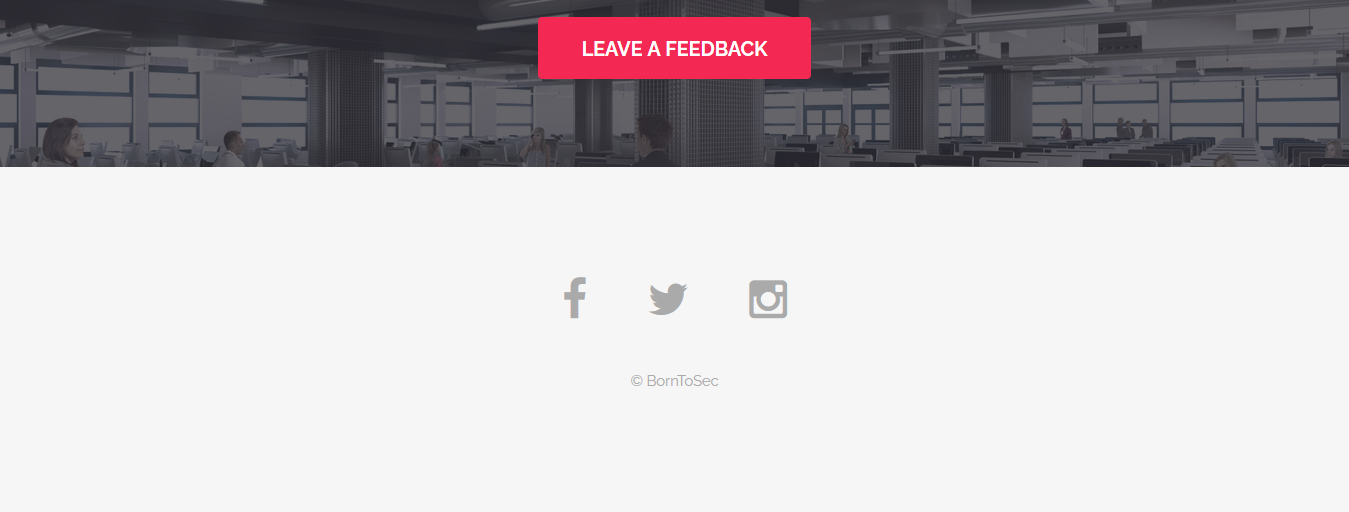
\includegraphics[width=.45\columnwidth]{08.Flag05/05-01.png}\label{fig: 05-01 - wtf}} \quad
    \subfloat[The Loud Bird]{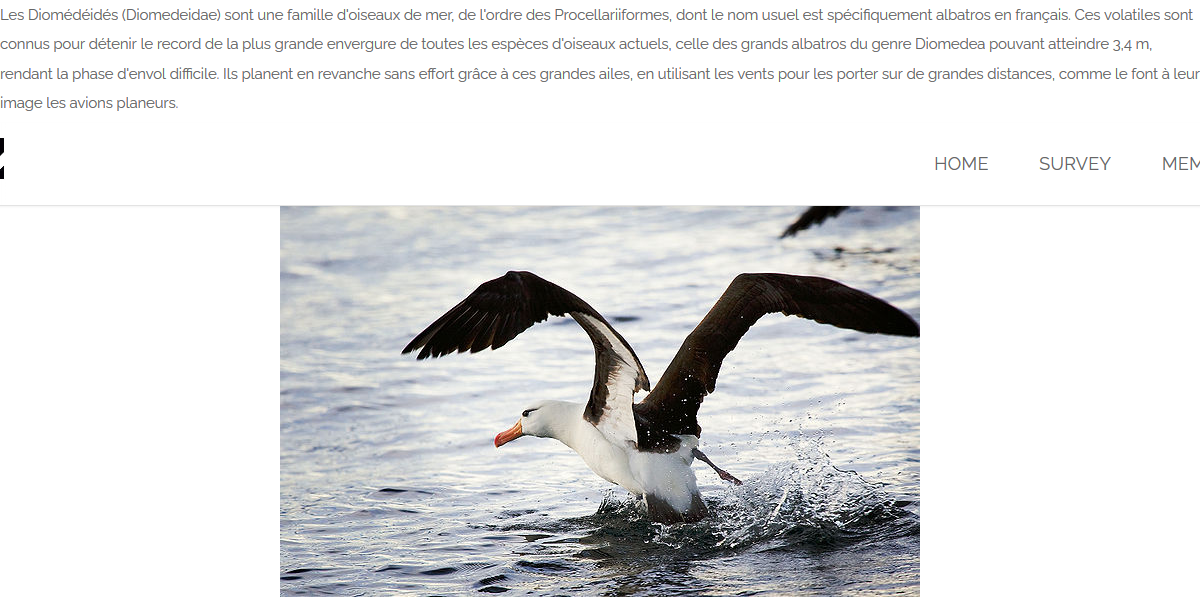
\includegraphics[width=.45\columnwidth]{08.Flag05/05-02.png}\label{fig: 05-02 - wrong}} \\
    \subfloat[Reload...]{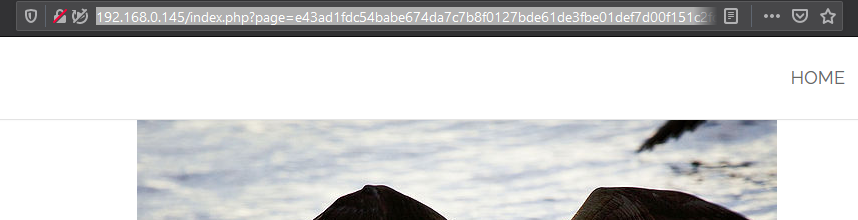
\includegraphics[width=.45\columnwidth]{08.Flag05/05-03.png}\label{fig: 05-03 - nope}} \quad
    \caption[Flag 05 Method]{Process to Capture the Spoof Flag} % The text in the square bracket is the caption for the list of figures while the text in the curly brackets is the figure caption
    \label{fig:flag05 method}
\end{figure}

\begin{itemize}
    \item Bash
    \item \href{https://curl.haxx.se/docs/manpage.html}{cURL}
    \item \href{https://owasp.org/www-community/attacks/Content_Spoofing}{Owasp}
    \item \href{https://www.freecodecamp.org/news/how-to-start-using-curl-and-why-a-hands-on-introduction-ea1c913caaaa/}{FreeCodeCamp}
\end{itemize}

\subsection{Remedy}

The HTTP Referer header is optional in HTTP and should not be sent unless
it is secure as explained on \href{https://www.w3.org/Protocols/rfc2616/rfc2616-sec15.html\#sec15.1.3}{W3Schools.com}.

Authors of services which use the HTTP protocol SHOULD NOT use GET based forms for the submission of sensitive data.

Servers can use POST-based form submission instead.

\textbf{Sources:}
\begin{itemize}
    \item \href{https://en.wikipedia.org/wiki/User\_agent}{Wikipedia - User Agent}
    \item \href{https://en.wikipedia.org/wiki/HTTP\_referer}{Wikipedia - HTTP Referer}
\end{itemize}
